% arara: pdflatex: {files: [MathSACpr2014]}
% !arara: indent: {overwrite: yes}
\chapter{Social Justice samples}\label{app:sec:socialJustic}

\pgfplotstableread{
	year    percentage
	1990	.135
	1991	.142
	1992	.148
	1993	.151
	1994	.145
	1995	.138
	1996	.137
	1997	.133
	1998	.127
	1999	.119
	2000	.113
	2001	.117
	2002	.121
	2003	.125
	2004	.127
	2005	.126
	2006	.123
	2007	.125
	2008	.132
	2009	.143
	2010	.151
	2011	.15
	2012	.16
	}\poverty

\emph{The problems below are samples from the Social Justice Work group}.

\Cref{app:tab:poverty} shows the percentage of people living in poverty in the U.S
(as defined by the government). Source: \href{http://www.census.gov/prod/2012pubs/p60-243.pdf}{http://www.census.gov/prod/2012pubs/p60-243.pdf}

\begin{table}[!htb]
	\centering
	\caption{Percentage of people living in poverty in the U.S}
	\label{app:tab:poverty}
	\pgfplotstabletypeset[
		every head row/.style={
			before row={\toprule},
			after row={\midrule}},
		every last row/.style={after row=\bottomrule},
		columns/year/.style={column name=Year,1000 sep={}},
		columns/percentage/.style={percentstyle,column name=Percentage,
			precision=1},
	]\poverty
\end{table}

Make a graph of the data and try to provide evidence (articles, news stories, policy, etc) 
for why these rate of poverty increased or decreased.  Once you completed the graph, 
draw in what \emph{you} think will happen in the next 10 years, give a reason to back up what you draw in.

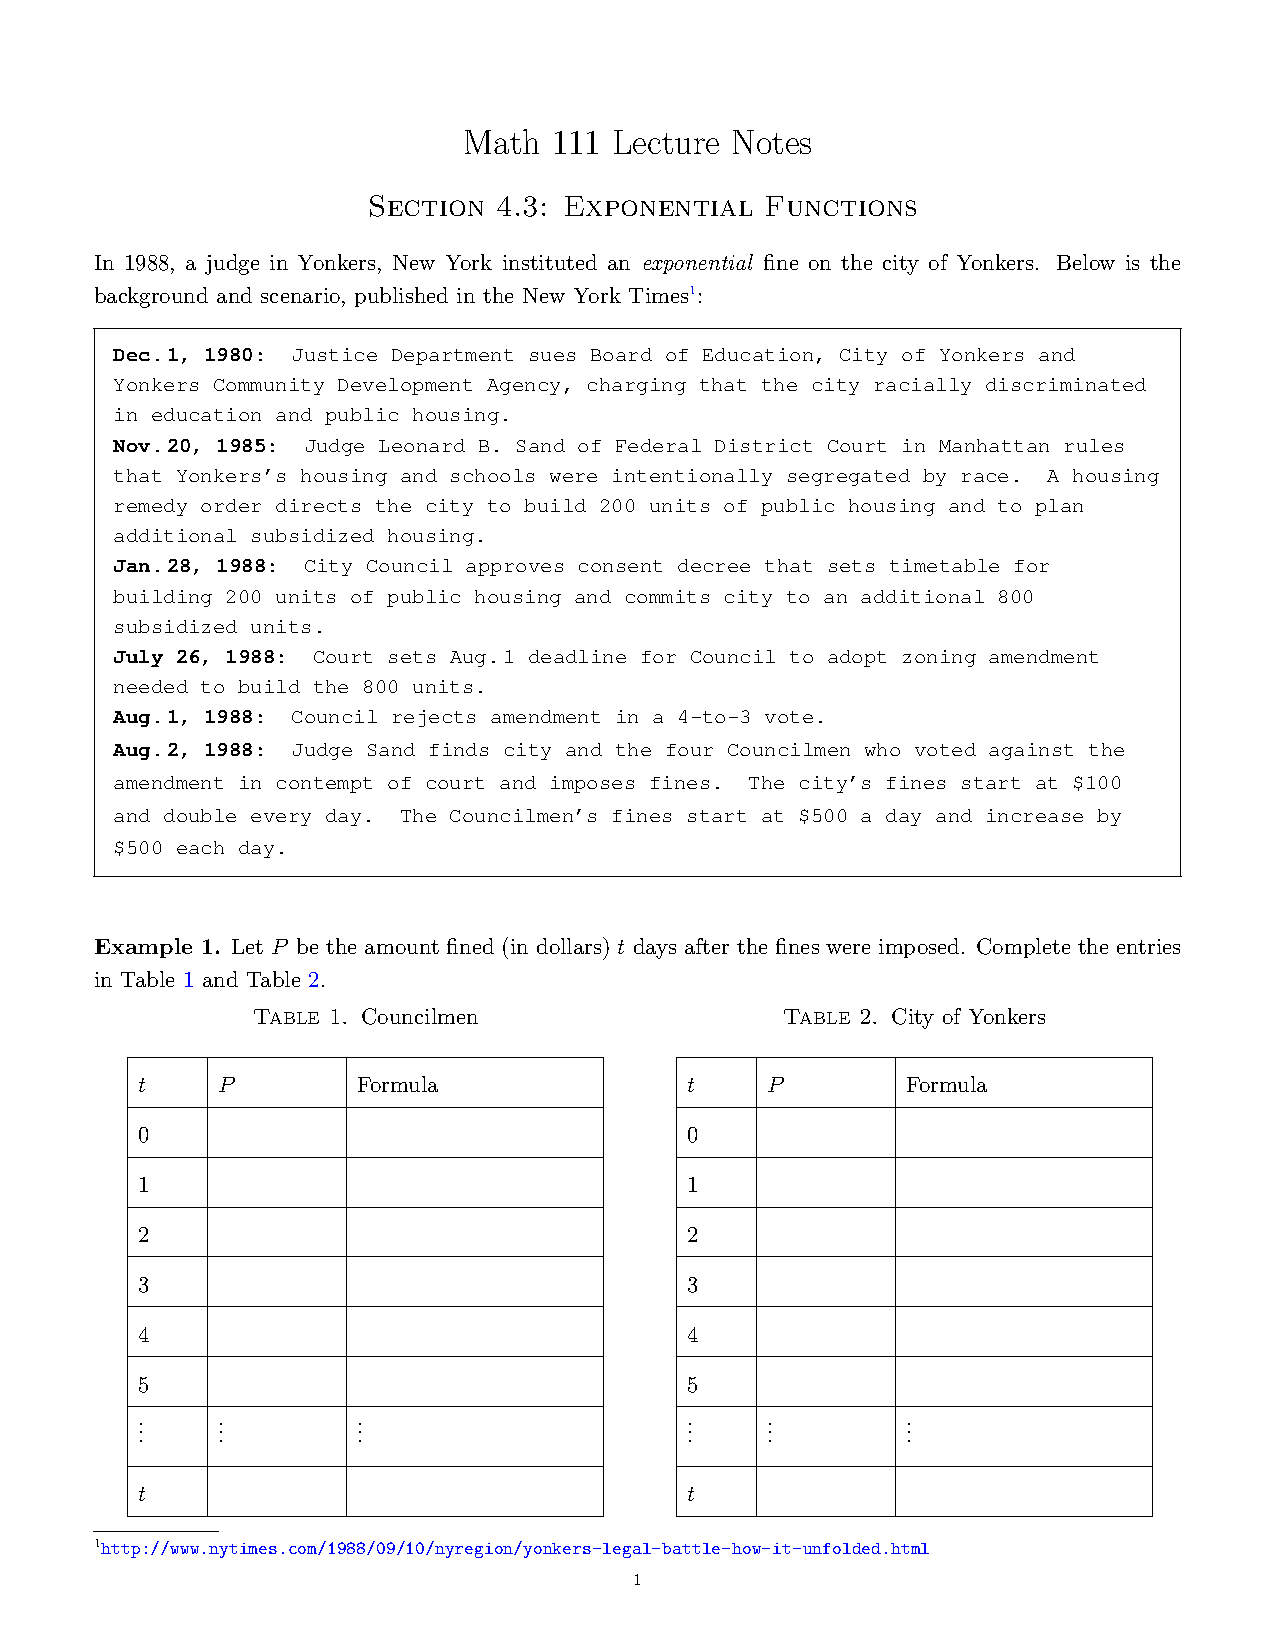
\includepdf[pages=-,pagecommand={\pagestyle{fancy}}]{./appendices/socialJusticeExample}
